
\begin{figure}[h]
  \centering
  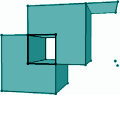
\includegraphics[width=10cm]{figs/teaser}
  \caption{The polyhedron viewer running on Windows. A coarse polygon 
    mesh is subdivided using the Quad-Triangle subdivision scheme.}
  \label{fig:viewer}
\end{figure}

Polyhedron data structures based on the concept of halfedges have been
very successful for the design of general algorithms on meshes.
Common practice is to develop such data structure from scratch, since
clearly a first implementation is at the level of a students homework
assignment. But then, these data structures consist almost entirely of
pointers for all sort of incidence informations. Maintaining them
consistently during mesh operations is not anymore a trivial
linked-list update operation. So, moving from a students exercise to a
reliable research implementation, including maintaining and optimizing
it, is a respectable software task.

What is common practice for simple data structures, such as linked
lists, should be common practice even more so for mesh data
structures, namely, to use a good, flexible, and efficient library
implementation. In \CC\, the \emph{Standard Template Library}, \stl,
is an excellent address for our analog example of the linked
lists~\cite{Austern:1999:GPS}, and we argue that
the Polyhedron data structure in \cgal\ is such a flexible mesh data
structure~\cite{k-ugpdd-99}, and it comes with a rich and versatile
infrastructure for mesh algorithms. \cgal, the 
\emph{Computational Geometry Algorithms Library}, is a 
\CC\ library available from \path|www.cgal.org|~\cite{fgkss-dccga-00}. 

We strongly believe that this tutorial with its wealth of
information will give a head start to new researches and implementations
of mesh algorithms. We also believe that it will raise the quality of
implementations. Firstly, it encourages the use of well tested and
over time matured implementations, e.g., \cgalpoly\ in its current
design was publicly released in 1999 and used since then. Secondly, it
documents good implementation choices, e.g., the example programs can
be used as starting points for evolutionary software development.
Thirdly, it offers easy access to additional functionality, such as
the efficient self intersection test, that otherwise could be
expandable in a research prototype.

The tutorial is organized around subdivision surfaces in a 
polyhedron viewer. The polyhedron viewer
(\figurename\ \ref{fig:viewer}) demonstrates the basic functionalities of
the \cgalpoly\ and some extended functionalities such as file I/O,
mesh superimposition, and trackball manipulation. Several subdivision
surfaces are supported in the polyhedron viewer, including
Catmull-Clark, Loop, Doo-Sabin, $\sqrt{3}$ and Quad-Triangle
subdivisions.  The tutorial shows how to implement subdivision
surfaces in two different mechanisms provided by \cgalpoly :
\emph{Euler operators} and \emph{modifier callback mechanism}.  A
$\sqrt{3}$ subdivision implementation is designed based on the Euler
operators and a Quad-Triangle subdivision implementation is designed
based on overloading the modifier.  Extended from the previous design,
a \emph{combinatorial subdivision library} (CSL) is then proposed with
increased sophistication and abstraction. CSL abstracts the geometry
operations from the refinements. Subdivisions in CSL are build from
refinement host with a template geometry policy. Several fundamental
refinement schemes are provided within CSL. They are instantiated with a
geometry policy that can be user defined.

The goal of this tutorial is to show how to use \cgalpoly\ on basic
graphics functionalities, such as rendering and interactive trackball
manipulation, \emph{and} how to design and implement algorithms around
meshes. Since connectivity and geometry operations are the primal
implementation components in mesh algorithms, subdivisions are chosen
to demonstrate both operations on \cgalpoly .  Hence, readers 
designing and implementing mesh algorithms other than subdivisions will
also benefit from the tutorial.

% ------------------------------------------------------------------------
\subsection*{Intended Audience}

The intended audience of the tutorial are researchers, developers or
students developing algorithms around polyhedron meshes. Knowledge of
the halfedge data structure and subdivisions are prerequisites.  Short
introductions of these two topics are given in the tutorial.  The
tutorial assumes familiarity with the \CC\ template mechanism and the
key concepts of generic programming~\cite{Austern:1999:GPS}.
